\documentclass{article}

% For title page
\usepackage[affil-it]{authblk}

% References
\usepackage{natbib}
\usepackage[normalem]{ulem} % No underlining in references

%\usepackage{appendix}
\usepackage{url} % not crucial - just used below for the URL

\usepackage{amsmath,amssymb,amsthm}
\usepackage{enumerate}

\usepackage{graphicx}
\graphicspath{ {images/} } % path pour figures

% for the networks
\def\layersep{2cm}
\usepackage{tikz}
\usepackage{verbatim}
\usetikzlibrary{decorations.pathreplacing}
\usetikzlibrary{shapes.geometric}

% Algorithms
\usepackage[ruled,vlined]{algorithm2e}

% to display the labels in the PDF, comment out before submission
%\usepackage{soul}
%\usepackage[color,notref,notcite]{showkeys}
%\definecolor{labelkey}{rgb}{0.6,0,1}



%%%%%%%%%%%%%%%%%%%%%%%%%%%%%%%%%%%%%%%%%%%%%%%%%%%%%%%%
%%%%%%%%%%%%%%%%%%%%%%%%%%%%%%%%%%%%%%%%%%%%%%%%%%%%%%%%


% Creation d'environnement
% \newtheorem{example}{Example}

% Allow equations to spread on different pages
% \allowdisplaybreaks


\linespread{1.25}


\begin{document}


\title{\bf Reliable Anomaly Detection using Variational Autoencoders}


\author[1]{St{\'e}phane Caron \thanks{Corresponding author: stephane.caron.9@ulaval.ca}}
\author[1]{Thierry Duchesne}
\author[2]{Fran\c{c}ois-Michel De Rainville}
\author[1]{Samuel Perreault}

\affil[1]{\small D{\'e}partement de math{\'e}matiques et de statistique, Universit{\'e} Laval, Qu{\'e}bec, Canada}
\affil[2]{\small Intact Insurance, Qu{\'e}bec, Canada}


\maketitle


\begin{abstract}
	In this paper, we propose an anomaly detection methodology that aims to detect anomalies among complex data, such as images, and that is based on a confidence level rather than on a certain threshold or metric. In order to do that, we demonstrate the usefulness of using variational autoencoders (VAE) to deal with complex data and also to have some kind of representation from which we can apply hypothesis testings. From our experiments, we can show that our approach is able to detect images that are outliers in a given dataset by only specifying a certain confidence level. By using this approach, the anomaly detection becomes feasible for real-world complex images and is also easier to maintain and interpret considering the detection is made on a confidence level rather than on a vague and possibly changing metric.
\end{abstract}

\textbf{Keywords:} autoencoder, hypothesis testing, confidence level, unsupervised.

% TO BE REMOVED
% \tableofcontents

\newpage

\section{Introduction}

Anomaly detection is a challenging topic that generated a lot of research in statistics, machine learning and more recently in computer vision. There are many applications of anomaly detection in fields such as cyber-intrusion, financial and insurance fraud detection, medical anomaly detection or industrial damage identification (\cite{Chandola07anomalydetection:}). An anomaly is defined by \cite{Zimek2017} as events, items or observations that differ significantly from the majority of the data. An anomaly, or what can also be called an outlier, is something intrinsic to many fields related with data because it is by nature, something interesting to extract or to remove from a given source of data.  It can be interesting to extract because it is what we are looking for in the problem or it could interesting to remove prior to another learning problem. \newline

One challenge with anomaly detection is that we often deal with unlabeled data, that means the problem usually needs to be tackled with an unsupervised approach. Another important challenge, especially with unsupervised approaches, is that those detection algorithms often need a threshold. That threshold allows us to take a decision regarding a certain anomaly. Finally, those challenges become even more problematic when dealing with complex data such as images. \newline

In that context highly complex data, neural networks are commonly used because their stacked layers are able to start from a complex input, like an image, and compress that information into smaller and richer representations. To deal with data without labels, a family of neural networks called the autoencoders are often used. Many applications of autoencoders exists in anomaly detection where the reconstruction error can used as a indicator of anomaly. However, those methodologies require a specific threshold, that can be difficult to define or can change in time. That is what \cite{An2015VariationalAB} tackled in their paper where the authors suggest a reconstruction probabilty, a measure that is more objective than the reconstruction error and does not require a threshold. However, the measure is still based on the reconstruction, where that could be problematic in the context of complex images compared to use a measure based on a more compressed representation.
\newline


In this study, we propose an approach that aims to simplify the threshold determination in the case of unsupervised anomaly detection. With this contribution, we are not proposing new methods, but simply put togheter the statistical theory behind hypotheses testing and autoencoders, more specifically variational autoencoders, to learn complex data structures and encode them into simpler representations. Those representations can then be tested with some confidence level, instead of a threshold based on a metric, to determine which observations are anomalies.

\section{Background} \label{background}

First, we will briefly describe the theory behind autoencoders and how it can be used in the context of anomaly detection. Then, we will describe one family of autoencoders, the variational autoencoders, and how its outputs can be used along with statistical hypothesis testing to detect anomalies.

\subsection{Autoencoders}

An autoencoder is an unsupervised neural network technique that aims to learn an efficient intermediate representation of an input (\cite{Goodfellow-et-al-2016}). To achieve this objective, the autoencoder has 2 components: an encoder and a decoder. The encoder receives an input $x$ and and converts it to a hidden representation $z$. The decoder receives a representation $z$ and decodes it back to retrieve as much as possible the input $x$. This structure is illustrated in the figure \ref{fig:basicAE}. Historically, autoencoders were known as a dimensionnalty reduction method, but it has now more applications by learning latent variables rich in informations.
\newline

\begin{figure}[h]
	\centering
	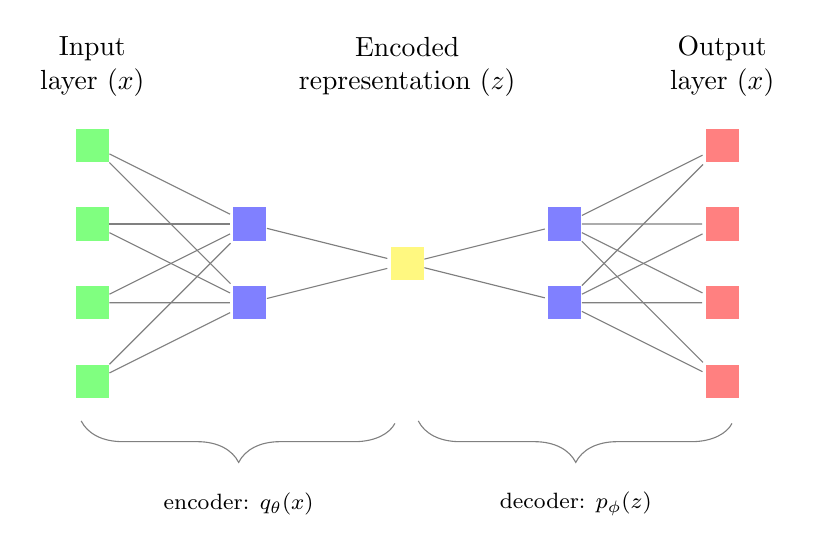
\begin{tikzpicture}[shorten >=1pt,draw=black!50, node distance=\layersep, square/.style={regular polygon,regular polygon sides=4}]
		\tikzstyle{every pin edge}=[<-,shorten <=1pt]
		\tikzstyle{neuron}=[square,fill=black!25,minimum size=17pt,inner sep=0pt]
		\tikzstyle{input neuron}=[neuron, fill=green!50];
		\tikzstyle{output neuron}=[neuron, fill=red!50];
		\tikzstyle{hidden neuron1}=[neuron, fill=blue!50];
		\tikzstyle{hidden neuron2}=[neuron, fill=blue!50];
		\tikzstyle{hidden rep}=[neuron, fill=yellow!50];
		\tikzstyle{annot} = [text width=4em, text centered]
		
		% Draw the input layer nodes
		\foreach \name / \y in {1,...,4}
		% This is the same as writing \foreach \name / \y in {1/1,2/2,3/3,4/4}
		\node[input neuron] (I-\name) at (0,-\y) {};
		
		% Draw the hidden layer nodes n.1
		\foreach \name / \y in {1,...,2}
		\path[yshift=-1cm]
		node[hidden neuron1] (H1-\name) at (\layersep,-\y cm) {};
		
		% Draw the encoded representation
		\foreach \name / \y in {1,...,1}
		\path[yshift=-1.5cm]
		node[hidden rep] (R-\name) at (2 * \layersep,-\y cm) {};
		
		% Draw the hidden layer nodes n.2
		\foreach \name / \y in {1,...,2}
		\path[yshift=-1cm]
		node[hidden neuron1] (H2-\name) at (3 * \layersep,-\y cm) {};
		
		% Draw the output layer
		\foreach \name / \y in {1,...,4}
		% This is the same as writing \foreach \name / \y in {1/1,2/2,3/3,4/4}
		\node[output neuron] (O-\name) at (4 * \layersep,-\y cm) {};
		
		% Connect input
		\foreach \source in {1,...,4}
		\foreach \dest in {1,...,2}
		\path (I-\source) edge (H1-\dest);
		
		% Connect representation
		\foreach \source in {1,...,2}
		\foreach \dest in {1,...,1}
		\path (H1-\source) edge (R-\dest);
		
		\foreach \source in {1,...,1}
		\foreach \dest in {1,...,2}
		\path (R-\source) edge (H2-\dest);
		
		% Connect outputs
		\foreach \source in {1,...,2}
		\foreach \dest in {1,...,4}
		\path (H2-\source) edge (O-\dest);
		
		% Annotate the layers
		\node[annot,above of=I-1, node distance=1cm] (hl) {Input layer ($x$)};
		\node[annot,above of=R-1, node distance=2.5cm][text width=8em] (hl) {Encoded \\ representation ($z$)};
		\node[annot,above of=O-1, node distance=1cm] (hl) {Output layer ($x$)};
		
		\draw [decorate,decoration={brace,mirror,amplitude=15pt},xshift=-4pt,yshift=-2cm]
		(0,-2.5) -- (4,-2.5) node [black,midway,yshift=-3em] 
		{\footnotesize encoder: $q_{\theta}(x)$};
		\draw [decorate,decoration={brace,mirror,amplitude=15pt},xshift=4pt,yshift=-2cm]
		(4,-2.5) -- (8,-2.5) node [black,midway,yshift=-3em] 
		{\footnotesize decoder: $p_{\phi}(z)$};
	
	\end{tikzpicture}
	\caption{Basic autoencoder structure example}
	\label{fig:basicAE}
\end{figure}

Autoencoders intuition is to build back the input $x$ by passing through the 2 components (encoder and decoder). As such, this kind of model does not need any target, so we say it is an unsupervised method. The training of the parameters is mainly done by minimizing the reconstruction error. The loss could then be given by a function in the form of:

$$
L(x, p_\phi{\{q_\theta(x)\}})
$$

\noindent where $q(x, \theta)$ is the encoder and $p(z,\phi)$ is the decoder function. The minimization of that loss function is done by gradient descent. For instance, the encoder and decoder parameters are gradually updated by taking the derivatives of the loss functions regarding to the different parameters:

\begin{equation} \label{optim}
\Theta \leftarrow \Theta-\epsilon*\frac{\partial L}{\partial\Theta}
\end{equation}

\noindent where $\epsilon$ is a learning weight that aims to control the size of the learning steps and $\Theta : \{\theta, \phi\}$ includes both encoder and decoder parameters.

Once the autoencoder is adequately trained, we can use the reconstruction error as an anomaly score. In \cite{10.5555/3086742}, that anomaly detection method is part of a catogory of algorithms based on linear or non-linear models. In this group of methods, we first fit a linear or non-linear model to the data and we use the reconstruction error, or the residual, as an anomaly score. Methods based on linear regression, principal components analysis (PCA), or matrix factorization are also part of this broad family of anomaly detection approaches. However, reconstruction is not the only criteria that can be used from autoencoders. In the next section, we cover a specific type of autoencoder, the variational autoencoder, and see how could we leverage another component as an anomaly score.

\subsection{Variational autoencoders} \label{background-vae}

The variational autoencoders (VAE) \cite{kingma2013autoencoding} have a slightly different approach than other kinds of autoencoders. In fact, instead of encoding a hidden representation of size $n$, it outputs two vectors of size $n$: a vector of means $\boldsymbol \mu$ and a vector of standard deviations $\boldsymbol \sigma$. Those two vectors are then used to generate a hidden representation that is sampled from a Gaussian distribution that gives this specific property to VAE, which is to have a continous latent representation. This is the main difference with other kinds of autoencoders. In other words, the basic autoencoders learn a reprensetation that "points" somewhere in the latent space, while VAE learns a representation that points to an "area", an area that is defined by the mean $\boldsymbol \mu$ and the standard deviation $\boldsymbol \sigma$ of the latent space. The figure \ref{fig:VAEstructure} illustrates the basic structure of a variational autoencoder. In the figure, we can see that the input data first pass through some layers (fully-connected or convolutional). At some point near the encoded representation, the layers are split into 2 components ($\mu$ and $\sigma$). The $z$ representation is sampled for a Gaussian distribution using sample the parameters $\mu$ and $\sigma$ corresponding to the values of those layers. Once we have the sampled representation, it is decoded back to the same size as the input. 

\begin{figure}[h]
	\centering
	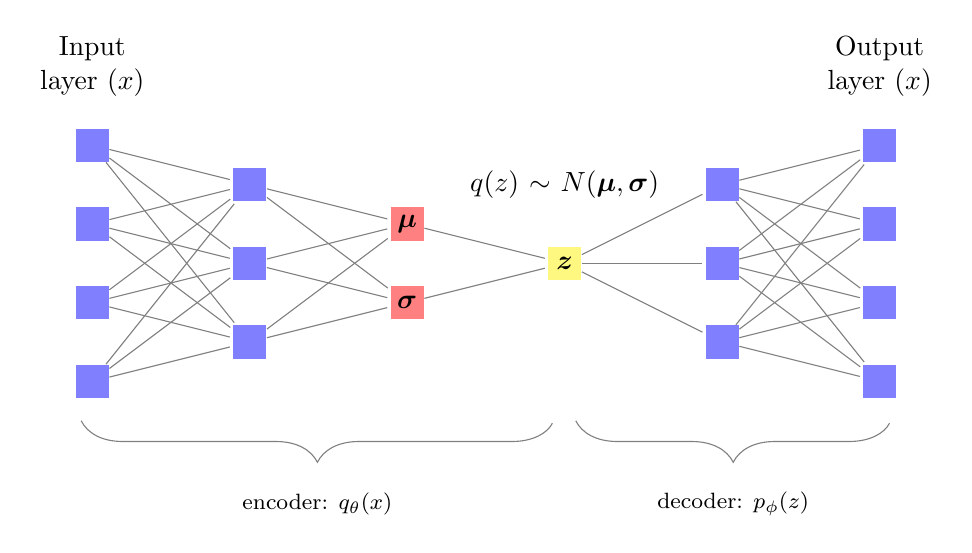
\begin{tikzpicture}[shorten >=1pt,draw=black!50, node distance=\layersep, square/.style={regular polygon,regular polygon sides=4}]
	\tikzstyle{every pin edge}=[<-,shorten <=1pt]
	\tikzstyle{neuron}=[square,fill=black!25,minimum size=17pt,inner sep=0pt]
	\tikzstyle{input neuron}=[neuron, fill=blue!50];
	\tikzstyle{output neuron}=[neuron, fill=blue!50];
	\tikzstyle{hidden neuron1}=[neuron, fill=blue!50];
	\tikzstyle{hidden neuron2}=[neuron, fill=blue!50];
	\tikzstyle{sample rep}=[neuron, fill=yellow!50];
	\tikzstyle{hidden rep}=[neuron, fill=red!50];
	\tikzstyle{annot} = [text width=4em, text centered]
	
	% Draw the input layer nodes
	\foreach \name / \y in {1,...,4}
	% This is the same as writing \foreach \name / \y in {1/1,2/2,3/3,4/4}
	\node[input neuron] (I-\name) at (0,-\y) {};
	
	% Draw the hidden layer nodes n.1
	\foreach \name / \y in {1,...,3}
	\path[yshift=-0.5cm]
	node[hidden neuron1] (H1-\name) at (\layersep,-\y cm) {};
	
	% Draw the mu and sigma layers
	\foreach \name / \y in {1,...,2}
	\path[yshift=-1cm]
	node[hidden rep] (R-\name) at (2 * \layersep,-\y cm) {};
	
	% Draw the encoded representation
	\foreach \name / \y in {1,...,1}
	\path[yshift=-1.5cm]
	node[sample rep] (S-\name) at (3 * \layersep,-\y cm) {};
	
	% Draw the hidden layer nodes n.2
	\foreach \name / \y in {1,...,3}
	\path[yshift=-0.5cm]
	node[hidden neuron1] (H2-\name) at (4 * \layersep,-\y cm) {};
	
	% Draw the output layer
	\foreach \name / \y in {1,...,4}
	% This is the same as writing \foreach \name / \y in {1/1,2/2,3/3,4/4}
	\node[output neuron] (O-\name) at (5 * \layersep,-\y cm) {};
	
	% Connect input
	\foreach \source in {1,...,4}
	\foreach \dest in {1,...,3}
	\path (I-\source) edge (H1-\dest);
	
	% Connect hidden 1 with mu and sigma
	\foreach \source in {1,...,3}
	\foreach \dest in {1,...,2}
	\path (H1-\source) edge (R-\dest);
	
	% Connect representation
	\foreach \source in {1,...,2}
	\foreach \dest in {1,...,1}
	\path (R-\source) edge (S-\dest);
	
	\foreach \source in {1,...,1}
	\foreach \dest in {1,...,3}
	\path (S-\source) edge (H2-\dest);
	
	% Connect outputs
	\foreach \source in {1,...,3}
	\foreach \dest in {1,...,4}
	\path (H2-\source) edge (O-\dest);
	
	% Annotate the layers
	\node[annot,above of=I-1, node distance=1cm] (hl) {Input layer ($x$)};
	\node[annot,above of=S-1, node distance=0cm][text width=8em] (hl) {$\boldsymbol z$};
	\node[annot,above of=S-1, node distance=1cm][text width=8em] (hl) {$ q(z) \sim N(\boldsymbol \mu, \boldsymbol \sigma)$};
	\node[annot,above of=R-1, node distance=0cm][text width=8em] (hl) {$\boldsymbol \mu$};
	\node[annot,above of=R-2, node distance=0cm][text width=8em] (hl) {$\boldsymbol \sigma $};
	\node[annot,above of=O-1, node distance=1cm] (hl) {Output layer ($x$)};
	
	\draw [decorate,decoration={brace,mirror,amplitude=15pt},xshift=-4pt,yshift=-2cm]
	(0,-2.5) -- (6,-2.5) node [black,midway,yshift=-3em] 
	{\footnotesize encoder: $q_{\theta}(x)$};
	\draw [decorate,decoration={brace,mirror,amplitude=15pt},xshift=4pt,yshift=-2cm]
	(6,-2.5) -- (10,-2.5) node [black,midway,yshift=-3em] 
	{\footnotesize decoder: $p_{\phi}(z)$};
	
	\end{tikzpicture}
	\caption{Variational autoencoder structure.}
	\label{fig:VAEstructure}
\end{figure}

When it comes to minimizing the loss, the variational autoencoder is also different from other autoencoders. In fact, there is another component added to basic reconstruction criterion. The loss function is then given by the sum of 2 components:

$$
L(x, p_\phi\{q_\theta(x)\}) + D_{KL}\big[q_\theta(z|x) || p(z)\big]
$$

where $D_{KL}$ is the Kullback-Leibler divergence. Its goal is to ensure that the encoded distribution $q(z)$ and a target distribution $p(z)$ are similar. The function $p(z)$ is a Gaussian distribution $N(0, I)$. In this kind of autoencoder, the hidden representation is stochastic because it is coming from a probability distribution. In order to simplify the derivatives in the backpropagation, we do a clever trick called the "reparametrization trick". In fact, it is possible for some distribution (such as the Gaussian), to separate the parameters ($\mu$ and $\sigma$) from the stochasticity. Concretely, we can express a normally-distributed variable as:

$$
z = \mu + \sigma \odot \epsilon
$$

\noindent where $\epsilon \sim N(0,1)$. In brief, that means that the $z$ layer in the figure \ref{fig:VAEstructure} is generated from the 2 parameters layers $\mu$ and $\sigma$ and a normal sample. The backpropagation then ignores the stochastic component, and derivates the parameters layers only, which simplifies at lot the optimization process.

\subsection{Hypothesis testing}

Hypothesis testing is a method of statistical inference. It aims to test a null hypothesis ($H_0$) versus an alternative hypothesis ($H_1$). In the context of anomaly detection, we could define hypotheses that allow us to test if a certain observation is coming from an expected population or not:
\newline

\noindent $\boldsymbol{H_0}$: $x_i$ comes from the population $P$ \\
$\boldsymbol{H_1}$: $x_i$ does not come from the population $P$
\newline

\noindent Once we have defined our hypothesis, we need a test method that will includes statistical assumptions about our sample. That generally consists of two components: an expected distribution and a metric. Having those two components, we can compute what we call a $p$-value. A $p$-value is defined as the probability, under null hypothesis, to observe the test statistic from the assumed distribution. When we have a small the $p$-value, it means that the null hypothesis may not adequatly explain the observation. The null hypothesis is then rejected when the value is less than a certain threshold $\alpha$, which is referred to as the level of significance. When the null hypothesis is true and the underlying random variable is continuous, then the probability distribution of the $p$-value is uniform on the interval [0, 1]. In this project, we are aiming to benefit from that level of significance rather than on a certain metric to detect anomalies.


\section{Methodology}

We propose an anomaly detection framework where we use the hidden representation of a variational autoencoder and transform that representation to a metric we can apply hypothesis testing and ultimatly detect anomalies with a level of significance.

\subsection{Approach}

In our approach, we suppose we have access to a dataset that contains mostly "normal", observations. Those "normal" observations could also be called \textit{inliers}. Considering we have access to such dataset, we use the variational autoencoders to learn the distribution of that "normal" population. That distribution is essentially contained in the hidden representation, or more specifically in the layers $\mu$ and $\sigma$ of the VAE. Like we described in the section \ref{background-vae}, VAE has the particularity of having a loss component applied to the latent representation, ensuring that the encoding follows a prior distribution, which is $N(0, I)$ in our case. Because of that, we can expect the $\mu$ and $\sigma$ layers of new inlier instances to have a small Kullbach-Leibler distance from a $N(0, I)$ distribution. Kullbach-Leibler (KL) distance is a measure a distance between 2 distributions. At the opposite, new outlier instances should have $\mu$ and $\sigma$ layers that are further from the prior distribution, so a greater KL distance. The proposed methodologie to compute $p$-values is describe in the algorithm \ref{anomaly_algo}.
\newline

\begin{center}
	\begin{algorithm}[H] \label{anomaly_algo}
		\SetAlgoLined
		\KwIn{Inliers dataset $x^{(j)}, j=1,...,m$, \\ Testing dataset with unknown anomalies $y^{(i)}, i=1, ..., n$}
		\KwOut{$p$-values for all test instances $p^{(i)}, i=1,...,n$}
	$\theta$, $\phi$ $\leftarrow$ train encoder ($q_{\theta}(x)$) and decoder ($p_{\phi}(z)$) VAE parameters\;
		\For{j=1 to m}{
			$\mu^{(j)} = p_{\theta}(x^{(j)})["mu"]$\;
			$\sigma^{(j)} = p_{\theta}(x^{(j)})["sd"]$\;
			$kl^{(j)}=kl\_distance(\mu^{(j)}, \sigma^{(j)})$
		}
		$kl\_sorted = sort(kl)$\;
		\For{i=1 to n}{
			$\mu^{(i)} = p_{\theta}(y^{(i)})["mu"]$\;
			$\sigma^{(i)} = p_{\theta}(y^{(i)})["sd"]$\;
			$kl_test^{(j)}=kl\_distance(\mu^{(i)}, \sigma^{(i)})$\;
			$p^{(i)} = Q_{kl\_sorted}(kl\_test)$ where Q is the quantile
		}
		\KwRet{$\boldsymbol{p}$}
		\caption{VAE anomaly detection algorithm}
	\end{algorithm}
\end{center}

In our proposed approach, the $p$-value is computed from an empirical distribution, which is the Kullbach-Leibler distances of all training instances. At the end, we are testing if a new observation is coming from the inliers population :

\begin{center}
$\boldsymbol{H_0}$: $y^{(i)}$ comes from the population $X$ \\
$\boldsymbol{H_1}$: $y^{(i)}$ does not come from the population $X$
\end{center}

\noindent Because we made the hypothesis that $X$ is mostly, if not entirely, inliers, we could rephrase our test :

\begin{center}
	$\boldsymbol{H_0}$: $y^{(i)}$ is an inlier \\
	$\boldsymbol{H_1}$: $y^{(i)}$ is an outlier
\end{center}

Finally, once we have the $p$-values of all instances of test dataset, we can use a level of significance $\alpha$ to conclude if it's an outlier (see the algorithm \ref{test_algo}).

\begin{center}
	\begin{algorithm}[H] \label{test_algo}
		\SetAlgoLined
		\KwIn{$p$-values for all test instances $p^{(i)}, i=1,...,n$, \\ level of significance $\alpha$}
		\KwOut{outlier indicators $o^{(i)}, i=1,...,n$}
		\For{i=1 to n}{
			\eIf{$p^{(i)} < \alpha$}{
				$o^{(i)}$ = $true$
			}
			{
				$o^{(i)}$ = $false$
			}
		}
		\KwRet{$\boldsymbol{o}$}
		\caption{Outlier decision algorithm}
	\end{algorithm}
\end{center}

\subsection{Adapt for complex data}

Parler de pourquoi utiliser les representation encoder pour le test au lieu de l'erreur de reconstruction. Peut-etre parler de la perceptual loss pour dealer avec une reconstruction difficile pour des images complex.

\subsection{Hypothesis testing advantages}

Parler du fait que c'est simple de definir un level of significance versus trouver une metric quelconque.

\section{Experiments}

\subsection{Datasets}

\subsection{Models tested}

\subsection{Discussion}

\section{Conclusion}

\section{Acknowledgment}

%\nocite{*} % pour citer toute la biblio, meme ceux pas cited dans le texte.
\bibliographystyle{apalike}
\bibliography{bibliography}

\end{document}